%!TEX root=paper.tex
  
\newpage
\section{Overhead of the \tool}
\label{sec:overhead}

To measure the performance overhead of the \tool, we have implemented an automated benchmarking system. It is open source and available online and can be tested by the reader. The benchmark downloads the latest version of the \zee API and installs it in a Docker container. Then it calls several selected endpoints for 500 times each, tracking the response times. The endpoints are called in three different configurations: 

	\begin{enumerate}
		\item With the dashboard disabled
		\item With the dashboard enabled but with the outlier detection deactivated
		\item With the dashboard enabled and the outlier treshold set to zero. This helps us measure the time usually spent in an outlier.
	\end{enumerate}



\Fref{fig:bench} shows using violin plots the distribution of times resulting from running the benchmark for three different endpoints on a quad-core machine, with Intel Core i5-4590 processor, @ 3.30GHz, 8G of RAM and 240GB SSD disk drive.


\begin{figure}[h!]
	\centering
	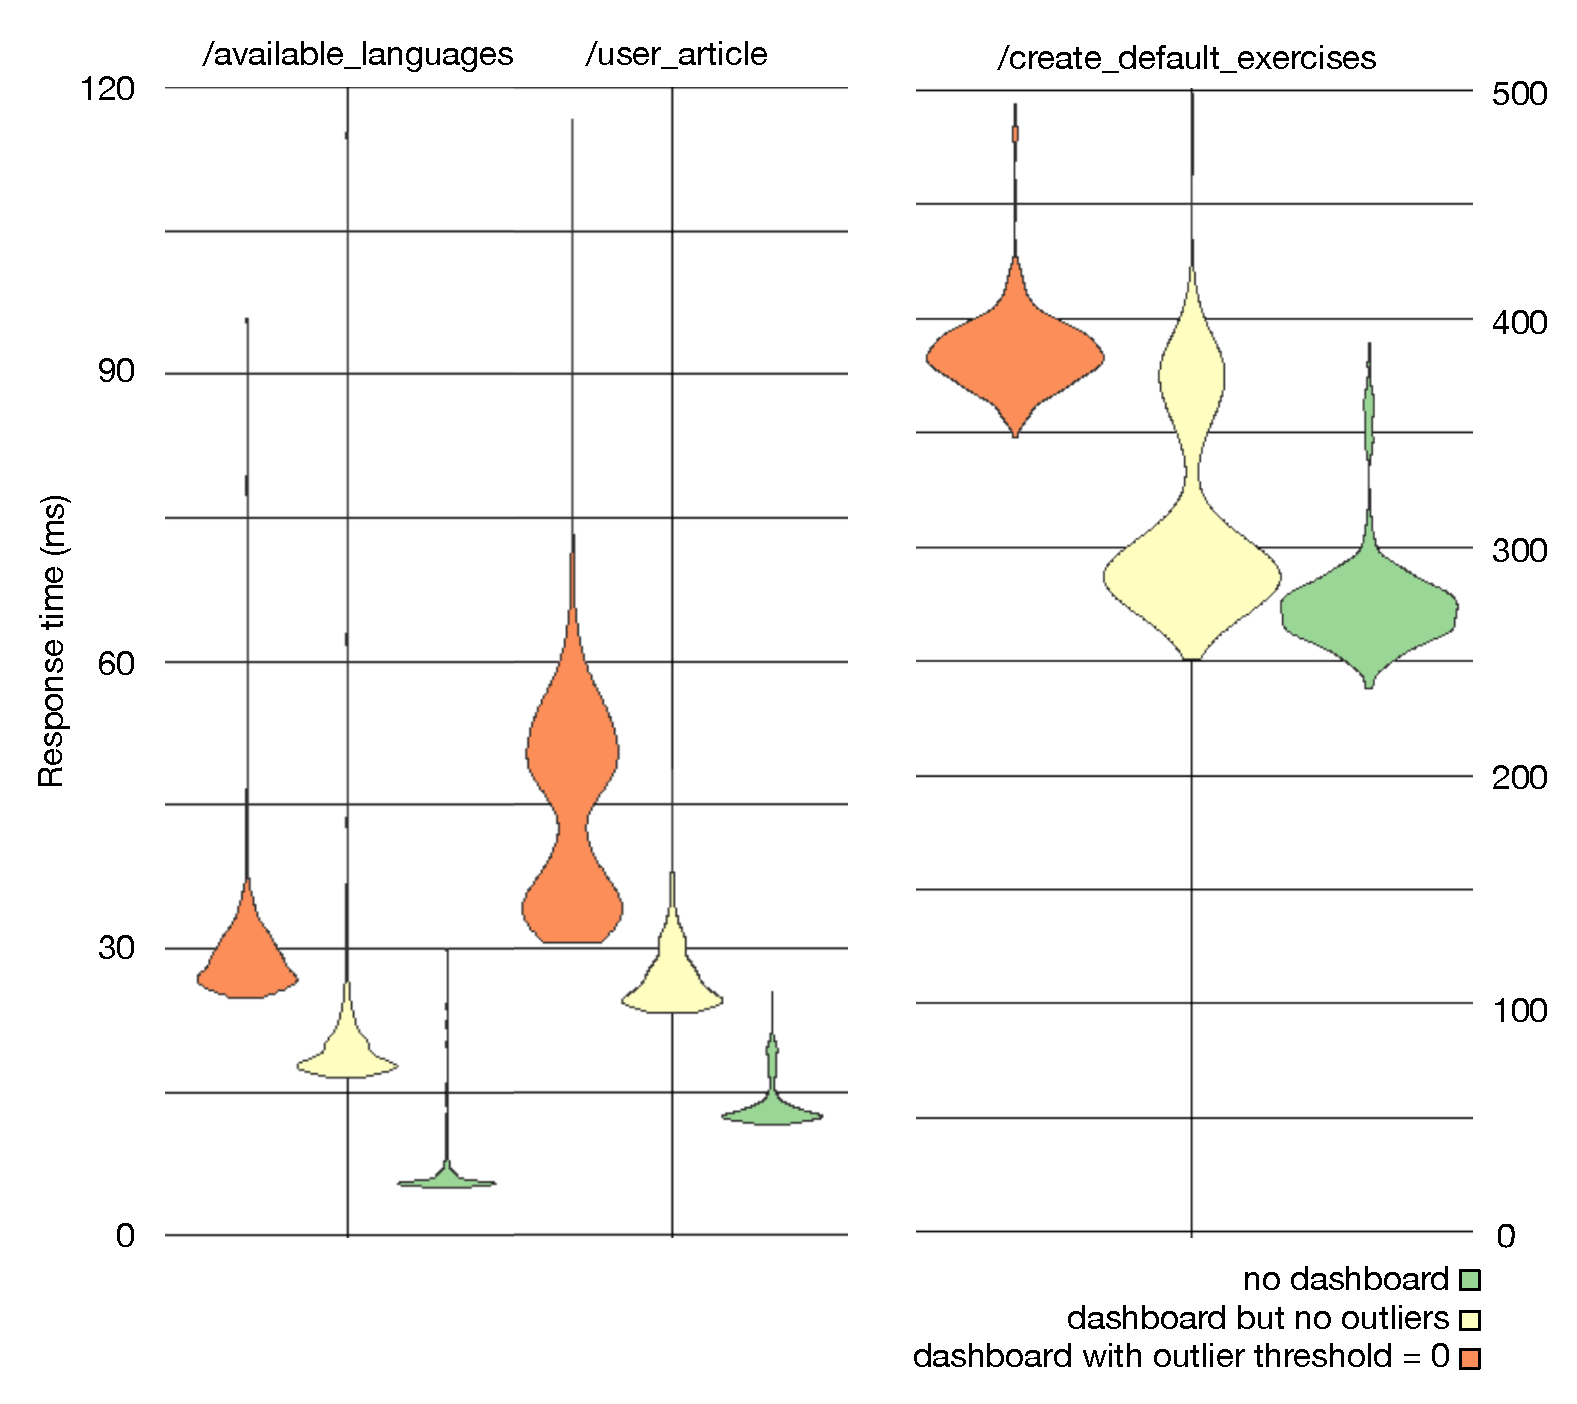
\includegraphics[width=\linewidth]{benchmark2.pdf}
	\caption{The distribution of response times when calling the three endpoints for 500 times in three conditions: no dashboard, dashboard but no outliers, dashboard and always outlier routine}
	\label{fig:bench}
\end{figure}


%!TEX root=paper.tex

\newcommand{\yes}{\checkmark}

\begin{table}[tb]
	
	\centering

	\begin{tabular}{rllrr}
		\toprule
		\bfseries Endpoint & \bfseries Dash. & \bfseries All Out. & \bfseries Mean (ms) & \bfseries SD (ms) \\

		\midrule

	         available\_languages  &    &	    &   6.3 &  2.3 \\ 
	         available\_languages  &  \yes &    &  19.9 &  5.6 \\ 
	         available\_languages  &  \yes &  \yes &  29.4 &  5.4 \\ \\ 

	                user\_article  &    &	    &  13.9 &  2.6 \\
	                user\_article  &  \yes &    &  26.9 &  3.2 \\
	                user\_article  &  \yes &  \yes &  44.8 & 10.0 \\ \\

	    create\_default\_ex...     &    &	    &  276.0 & 22.4 \\ 
	    create\_default\_ex...     &  \yes &    & 313.6 & 43.2 \\
	    create\_default\_ex...     &  \yes &  \yes & 385.3 & 16.9 \\
	
		\bottomrule

	\end{tabular}
	\caption{Response times for three endpoints run 500 times in three different conditions each. Dash. = with dashboard. All Out. = every call being considered an outlier}
	\label{tab:benchmark}

\end{table}





Observation -- not easy to benchmark this... it's flask on top of python communicating with 

- this introspection, which looks up endpoints, happens only once at the startup of the service, so it is going to affect the API startup performance, but not the actual endpoint performance. In our case, the overhead here was quite small: TO MEASURE


  